%%%%%%%%%%%%%%
\section{Tuesday 28 August:  Scan Conversion of a Line Segment}
%%%%%%%%%%%%%%%%

{\bf Simplifying Assumptions}

1-pixel-thick line on a B\&W display (monochrome)

$m \in [-1,1]$.  More elaborate code can deal with other slopes.

Line segment described by two integer endpoints (endpoints fall exactly on pixels) $(x_s,y_s), (x_e,y_e)$

\

\hfil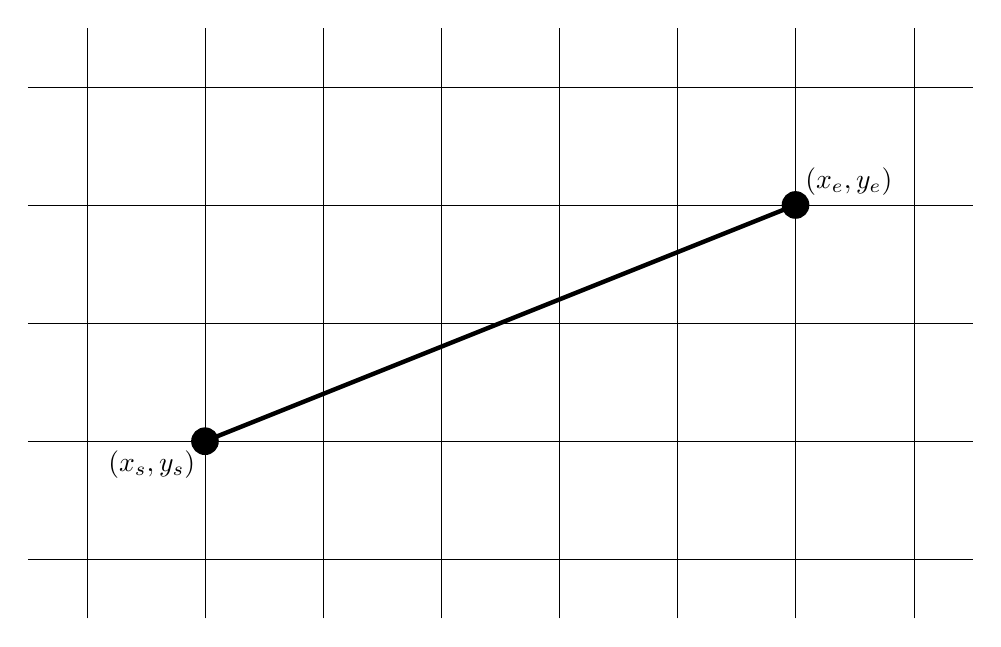
\begin{tikzpicture}[x=15mm, y=15mm]
	\foreach \i in {0,1,2,...,4}{
		\draw [ultra thin] (-0.5,\i) -- (7.5,\i);
	}
	\foreach \i in {0,1,2,...,7}{
		\draw [ultra thin] (\i,-0.5) -- (\i,4.5);
	}
	\coordinate (S) at (1,1);
	\coordinate (E) at (6,3);
	\fill (S) circle (5pt) node [below left] {$(x_s,y_s)$};
	\fill (E) circle (5pt) node [above right] {$(x_e,y_e)$};
	\draw [ultra thick] (S) -- (E);
\end{tikzpicture}

{\bf Main Idea}:  Activate one pixel per column from $x_s$ to $x_e$.  

\

\hfil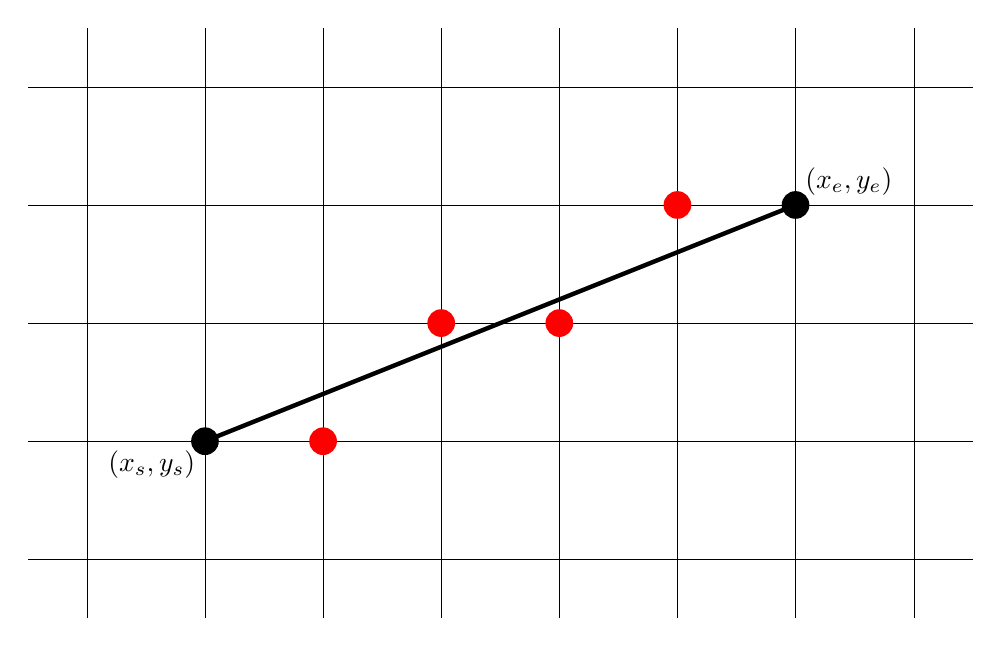
\begin{tikzpicture}[x=15mm, y=15mm]
	\foreach \i in {0,1,2,...,4}{
		\draw [ultra thin] (-0.5,\i) -- (7.5,\i);
	}
	\foreach \i in {0,1,2,...,7}{
		\draw [ultra thin] (\i,-0.5) -- (\i,4.5);
	}
	\coordinate (S) at (1,1);
	\coordinate (E) at (6,3);
	\fill (S) circle (5pt) node [below left] {$(x_s,y_s)$};
	\fill (E) circle (5pt) node [above right] {$(x_e,y_e)$};
	\draw [ultra thick] (S) -- (E);
	\fill [red] (2,1) circle (5pt);
	\fill [red] (3,2) circle (5pt);
	\fill [red] (4,2) circle (5pt);
	\fill [red] (5,3) circle (5pt);
\end{tikzpicture}

{\bf Simple, but Slow, Algorithm}

$m = (y_e - y_s) / (x_e - x_s)$

$b = y_s - m \cdot x_s$

for $x$ from $x_s$ to $x_e$ {\color{red} \it (inclusive)}

\qquad color pixel at $(x, \lfloor m \cdot x + b + 0.5 \rfloor)$

\

The problem with this algorithm that is the $m \cdot x$, floating-point multiplication, is really computationally expensive, usually six cycles, while addition is relatively cheap, usually one cycle.  

\

Rendering algorithms have to be as fast as possible, because they run billions of times.  

\

{\bf Basic Incremental Algorithm (DDA, Digital Differential Analyzer)}

$m = (y_e - y_s) / (x_e - x_s)$

$b = y_s - m \cdot x_s$

$x_0 = x_s$

$y_0 = y_s$

for $i$ from 1 to $(x_e - x_s)$

\qquad $(x_{i+1}, y_{i+1}) = (x_i + 1, y_i + m)$

\qquad color pixel at $(x_i+1, \lfloor y_{i+1} + 0.5 \rfloor )$ 

\

{\bf Midpoint Algorithm (Besenham)}

Developed for pen plotter.

Bottleneck was algorithm and computational speed, not hardware speed.

\

Simplifying assumption:  $m \in [0,1]$

\

Main idea

\qquad Move either E or NE in each move.  

\qquad Choose based on value of decision variable, $d$, which lets us choose betwen E and NE.  

\

\

\hfil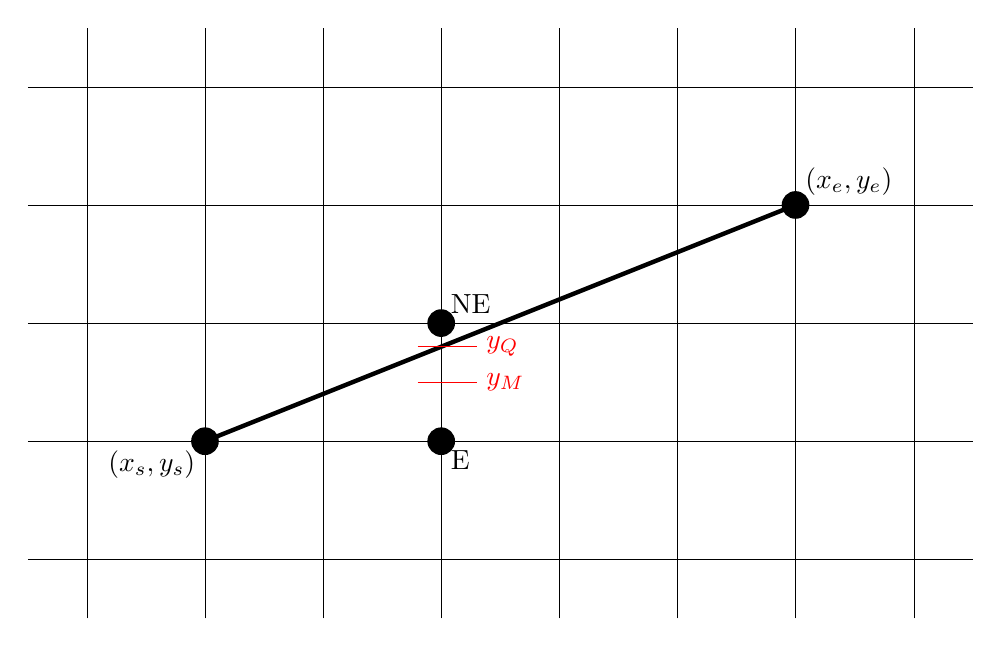
\begin{tikzpicture}[x=15mm, y=15mm]
	\foreach \i in {0,1,2,...,4}{
		\draw [ultra thin] (-0.5,\i) -- (7.5,\i);
	}
	\foreach \i in {0,1,2,...,7}{
		\draw [ultra thin] (\i,-0.5) -- (\i,4.5);
	}
	\coordinate (S) at (1,1);
	\coordinate (E) at (6,3);
	\fill (S) circle (5pt) node [below left] {$(x_s,y_s)$};
	\fill (E) circle (5pt) node [above right] {$(x_e,y_e)$};
	\draw [ultra thick] (S) -- (E);
	\draw [red] (2.8,1.8) -- (3.3,1.8) node [right, red] {$y_Q$};
	\draw [red] (2.8,1.5) -- (3.3,1.5) node [right, red] {$y_M$};
	\fill (3,1) circle (5pt) node [below right] {E};
	\fill (3,2) circle (5pt) node [above right] {NE};
\end{tikzpicture}

Notation:   $Q$ for {\it crossing}, $M$ for {\it midpoint}.

\

{\bf Algorithm}

$d = y_Q - y_M$.  

Look at sign of $d$.  

Move NE when $d$ is positive.

Move E otherwise.  

\

{\bf Computing $d$}

Initialize $d = m - 0.5$

Increment:

\qquad for E moves:  $d = d+m$

\qquad for NE moves:  $d = d + m - 1$

\

Here's how Midpoint is cheaper than DDA:  We can change everything to integers and not have any floats.  

\

{\bf Make Everything Integers}

Scale everything by $2 \Delta x$, so that $m - 0.5$ becomes an integer.  

$d = 2 \Delta y - \Delta x$

East increment:  $d = d + 2 \Delta y$

NE increment:  $d = d + 2 \Delta y - 2 \Delta x$

\

These methods aren't what we use today.  Probably triangle scan conversion.  

